\section{Benchmark and Analysis}

\subsection{Experimental Setup}
\noindent \textbf{Simulation Environments}.
We evaluate our system in outdoor scenarios using the high-fidelity simulator Unreal Engine 4.27~\cite{ue}. The benchmark comprises four diverse large-scale environments: Downtown, Cabinlake, Neighborhood, and Venice. These environments contain various terrain types including villages, cities, parks, forests, roads, seas, and mountains, covering areas from 160,000 to 562,500 $\mathrm{m}^2$. 
The benchmark includes 85 task episodes involving 25 target object categories, described by open-ended task instructions that incorporate environmental semantics (e.g., boats on water, cars on roads).
The environments, word cloud of task instructions, and representative objects are shown in \fig\ref{fig:simenv}.


\noindent \textbf{Metrics}.
Following prior works~\cite{xiao2025uav,ji2025towards}, we adopt five common metrics: Success Rate (SR), Oracle Success Rate (OSR), Success weighted by inverse Path Length (SPL), Distance to Goal (DTG), and Flight Time (FT). SR measures whether the drone stops within a threshold distance of the goal object. OSR checks if the drone comes within this threshold at any point during the episode. SPL evaluates navigation efficiency by weighting success with the ratio of optimal to actual path length. DTG computes the final Euclidean distance to the target object. FT records the total flight time per episode from takeoff to task termination, including the VLM inference time. Note that FT is a critical metric for real-world deployment that has been overlooked in previous works.

\noindent \textbf{Baselines}. 
We evaluate \sysname against a diverse set of drone-based object navigation methods. 
\textbf{PRPSearcher}~\cite{ji2025towards} is a motion primitive-based pipeline that maintains a semantic attraction map and leverages VLM reasoning for discrete action selection.
\textbf{UAV-on}~\cite{xiao2025uav} uses a VLM to convert RGB frames into text, augments them with depth and pose history, and passes the structured prompt to an LLM to produce discrete navigation commands. \textbf{FlySearch}~\cite{pardyl2025flysearch} overlays RGB images with a coordinate grid and queries a VLM to select the next target location. \textbf{STARSearcher}~\cite{luo2024star} relies purely on geometric information to guide exploration, using a hierarchical planner to seamlessly switch between exploring unknown areas and inspecting surface regions. 
\textbf{Human Agent} represents the average performance of three professional drone operators who completed over 20 hours of training in the simulator, establishing the human expert baseline.


\noindent \textbf{Implementation Details}. 
% metricx具体阈值的设置, 用了qwen的模型，参考3dmem，无人机的速度，加速度等，参考fuel 
We simulate a drone in AirSim~\cite{shah2017airsim} equipped with a LiDAR sensor (10 m range) and three RGB cameras (facing front, left, right), each with a $90^\circ \times 60^\circ$ field of view. Dynamic limits are set to $v_{m}=2.0$ m/s, $\mathbf{a}_{m}=1.5$ m/s$^2$, and $\omega_{m}=0.9$ rad/s. Our system uses Grounding-DINO~\cite{liu2024grounding} for object detection and SAM2~\cite{ravi2024sam2} for segmentation. All methods employ Qwen-VL-Max API~\cite{yang2025qwen3} as the VLM for reasoning to ensure fair comparison. Semantic threshold $\rho$ is set to 0.15. For evaluation metrics, the SR and OSR adopt a distance threshold of $5\text{m}$, while each task is limited to a maximum of $50$ VLM queries. Each task episode runs three times per method on an identical computer with an Intel Core i7-14700KF, GeForce RTX 4070 12G, and 32 GB memory. We employ an open-source solver~\cite{solver} to solve the optimization problem in \S\ref{V-C}.



\begin{table}[t]
\caption{\textbf{Overall Performance Comparison}. Best results in \colorbox{cyan!15}{cyan}, second-best in \colorbox{violet!15}{violet}, and Human Agent in \colorbox{gray!20}{gray}.}
\vspace{-5pt}
\centering
\renewcommand{\arraystretch}{1.3}
\resizebox{\columnwidth}{!}{%
\begin{tabular}{lcccccc}
\toprule
\textbf{Method} & \textbf{SR $\uparrow$} & \textbf{OSR $\uparrow$} & \textbf{SPL $\uparrow$} & \textbf{DTG $\downarrow$} & \textbf{FT $\downarrow$} \\
\midrule
Human Agent &\cellcolor{gray!20} 80.5 &\cellcolor{gray!20} 81.7 & \cellcolor{gray!20}61.7 & \cellcolor{gray!20}18.8 & \cellcolor{gray!20} 24.6 \\
\midrule
% Random & 4.9 & 15.8 & 3.3 & \cellcolor{violet!10}59.1 & \textbf{\cellcolor{cyan!15}62.6} \\
PRPSearcher & \cellcolor{violet!10}24.0 & 26.6 & \cellcolor{violet!10}19.3 & 90.2 & 324.6 \\
UAV-on & 7.4 & 33.3 & 3.8 & \cellcolor{violet!10}64.9 & 364.13 \\
FlySearch & 20.3 & \cellcolor{violet!10}34.2 & 8.6 & 137.5 & 767.7 \\
STARSearcher & 2.4 & 4.9 & 1.1 & 103.5 & \cellcolor{violet!10}296.7 \\
% \midrule
\sysname(Ours) &\textbf{\cellcolor{cyan!15}73.1} & \textbf{\cellcolor{cyan!15}80.5} & \textbf{\cellcolor{cyan!15}42} & \textbf{\cellcolor{cyan!15}11.6} & \textbf{\cellcolor{cyan!15}120.8} \\
\bottomrule
\end{tabular}
}
\label{tab:overall}
\vspace{-18pt}
\end{table}


\subsection{Benchmark Results}\label{VI-B}
\subsubsection{Quantitative Results}
We evaluate \sysname across all scenes as summarized in \tab~\ref{tab:overall}. \sysname demonstrates superior performance across diverse environments over all baseline methods except the Human Agent. Notably, \sysname achieves a 49.1\% improvement in SR compared to the strongest baseline PRPSearcher. 
Among the baselines, STARSearcher exhibits the poorest performance in SR, as it requires close-range inspection of all occupied voxel surfaces. 
While this exhaustive strategy excels in small-scale environments, it makes the drone prone to becoming trapped in structurally complex regions. UAV-on also achieves low SR, as its reliance on salient visual features for decision-making leads to limited active exploration capability.

\begin{figure*}[t]
    \centering
    \setlength{\abovecaptionskip}{-3pt}  % 默认约为 10pt
    
    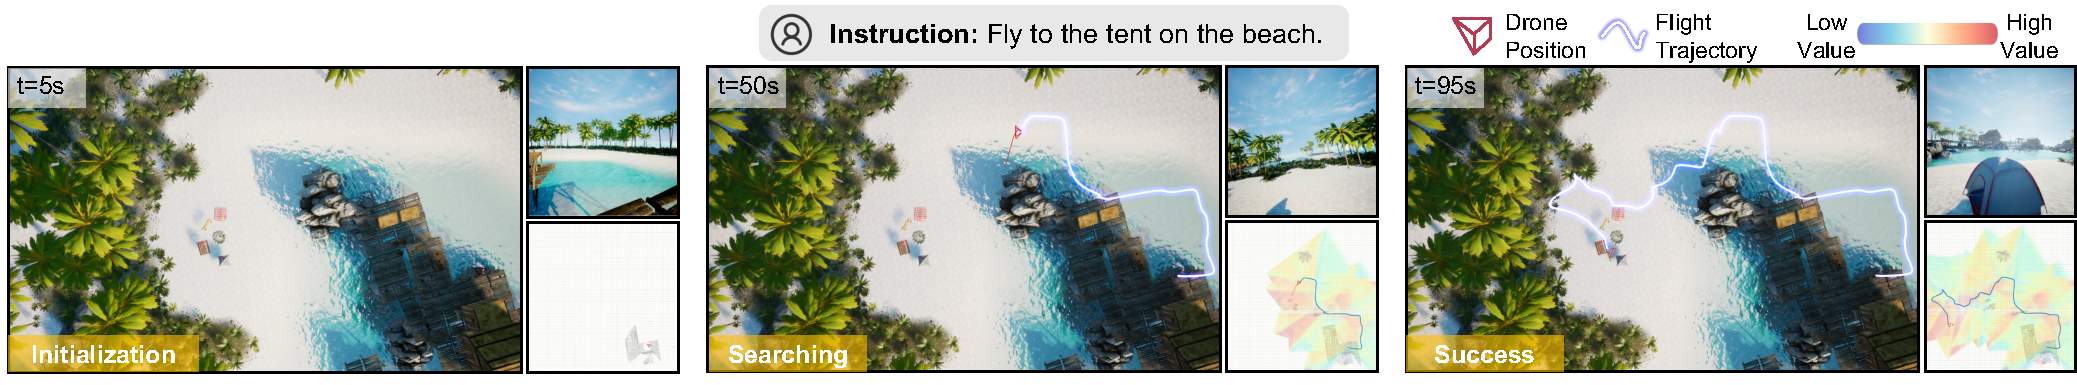
\includegraphics[width=0.98\linewidth]{figures/simdemo.pdf}
    \caption{Example qualitative results of \sysname in the Cabinlake environment. The left subfigure shows the top-down view of the scenario. The upper right shows the first-person view of drone and the lower right shows the 3D value map.}
    \label{fig:simdemo}
    \vspace{-12pt}
\end{figure*}
\begin{table}[t]
\caption{Ablation Study on Key Modules.}
\vspace{-5pt}
\centering
\renewcommand{\arraystretch}{1.25}
\resizebox{\columnwidth}{!}{%
\begin{tabular}{lccccc}
\toprule
\textbf{Method}
& \textbf{SR $\uparrow$}
& \textbf{OSR $\uparrow$}
& \textbf{SPL $\uparrow$}
& \textbf{DTG $\downarrow$}
& \textbf{FT $\downarrow$} \\
\midrule
RecTask1              &  {59.3} &  {68.8} &  {40.7} &  {25.6} & 128.7 \\
RecTask2           &  {31.2} &  {38.4} &  {12.5} &  {65.1} & 135.6 \\
\midrule
Value-greedy              &  {16.2} &  {18.3} &  {5.5} &  {105.6} & 312.7 \\
Scalarization              &  {33.2} &  {38.9} &  {17.5} &  {54.2} & 239.4 \\
Two-stage           &  {58.9} &  {63.4} &  {32.5} &  {21.4} & 198.2 \\
\midrule
\rowcolor{gray!20}
\sysname  &  \textbf{73.1} &  \textbf{80.5} &  \textbf{42.0} &  \textbf{11.6} & \textbf{120.8} \\
\bottomrule
\end{tabular}%
}
\label{tab:ablation}
\vspace{-12pt}
% \vspace{0.25em}
\end{table}
Navigation accuracy is further assessed using DTG. \sysname achieves the lowest DTG across all methods.
This advantage stems from the proposed ADTR module, which constructs task-aware keyframes to capture both object-level details and scene-level contextual information, thereby enabling more reliable VLM-based decision-making. 
In contrast, baseline methods fail to consistently integrate both geometric and semantic information into path planning, causing the drone to become disoriented in expansive environments. Note that \sysname surpasses even the Human Agent, as it can obtain the target's 3D position to determine the stopping location more precisely. 
These results demonstrate that \sysname enables accurate target localization in open-world outdoor environments.


We further evaluate navigation efficiency using SPL and FT.
Results indicate that baseline methods demand substantially longer flight times and travel distances to complete tasks. PRPSearcher achieves the highest SR among baselines, yet requires an average FT of 324.6s, 2.5 times longer than \sysname.
This is because PRPSearcher's stop-and-infer behavior, where the drone needs to hover during VLM inference, significantly disrupts flight continuity and reduces efficiency.
In contrast, our asynchronous architecture allows the VLM reasoning and planning processes to operate without blocking each other, achieving more smooth and efficient flight.
 

\subsubsection{Qualitative Results}
As shown in \fig\ref{fig:simdemo}, we present a representative task episode to illustrate the qualitative results of \sysname, including the executed flight trajectory and 3D value map visualization. Given the instruction ``Fly to the tent on the beach'', the drone starts near a cabin, then generates a smooth trajectory to quickly explore high-value regions, and successfully locates the target object on the beach. The value map shows that \sysname assigns higher values to regions more likely to contain the target object. Moreover, the flight trajectory prioritizes these high-value regions while avoiding revisits to explored areas, demonstrating the spatial consistency of our approach.


\subsection{Ablation Study}
\subsubsection{Ablation Study on ADTR}
In \tab~\ref{tab:ablation}, we evaluate the impact of ADTR on system performance. We design two variants: (i) RecTask1, which replaces coverage-aware keyframe construction with the most recent egocentric observations for Task 1 VLM queries; and (ii) RecTask2, which directly feeds raw observations to the VLM to determine whether the target object is visible and within the success threshold distance. All other components remain identical to \sysname. 
RecTask1 shows significant degradation, with SR dropping from 73.1\% to 59.3\%. This occurs because relying solely on recent observations results in both insufficient spatial coverage and temporal redundancy across consecutive frames, limiting the VLM's spatial reasoning effectiveness.
RecTask2 exhibits even larger degradation, with SR decreasing by 41.9\%. This is expected since VLM cannot reliably estimate the distance to the target object from raw image, leading to premature task termination, particularly in complex scenes with severe occlusion.
These results confirm that our ADTR module is critical for the effectiveness of the downstream planner by providing compact and informative content for VLM reasoning.


\begin{table}[t]
\caption{Average Computation Time ({\normalfont ms}) of Key Components.}
\vspace{-5pt}
\centering
\renewcommand{\arraystretch}{1.2}
\resizebox{\columnwidth}{!}{%
\begin{tabular}{lccccccc}
\toprule
\multirow{3}{*}{\textbf{Scene}} & \multicolumn{3}{c}{\textbf{ADTR \S\ref{IV}}} & \multicolumn{3}{c}{\textbf{SGCP \S\ref{V}}} \\
\cmidrule(lr){2-4}\cmidrule(lr){5-7}

 & \makecell{\textbf{Task 1}\\\textbf{\S \ref{IV-B}}}
 & \makecell{\textbf{Task 2}\\\textbf{\S \ref{IV-B}}}
  & \makecell{\textbf{Value.}\\\textbf{\S \ref{IV-C}}}
 & \makecell{\textbf{Front.+VP.}\\\textbf{\S \ref{V-A},\ref{V-B}}} 
 & \makecell{\textbf{Global}\\\textbf{\S \ref{V-C}}}
 & \makecell{\textbf{Local}\\\textbf{\S \ref{V-D}}}\\
\midrule
Cabinlake
& 3041 & 4711 & 5 & 1.3 & 24.3 & 0.2  \\
Downtown
& 3418 & 4288 & 12 & 2.2 & 13.2 & 0.2  \\
Neighborhood
& 4285 & 3950 & 8 & 2.4 & 30.4 & 0.4 \\
Venice
& 3721 & 5270 & 7 & 3.2 & 14.9 & 0.9 \\
\bottomrule
\end{tabular}%
}
\label{tab:comptime}
\vspace{-10pt}
\end{table}
\subsubsection{Ablation Study on SGCP}
We also evaluate the effectiveness of the SGCP module by comparing three variants: (\textit{i}) Value-greedy, which chooses the frontier with the highest semantic value as the next goal; 
(\textit{ii}) Scalarization, which always selects the frontier with the highest utility score (\ie, value/distance) as the next goal;
and (\textit{iii}) Two-stage~\cite{zhang2025apexnav}, which selects a subset of high-value frontiers by threshold and solves a Traveling Salesperson Problem (TSP) tour over the subset. All other components remain identical to \sysname. 
As shown in \tab~\ref{tab:ablation}, all variants show performance decline across all metrics.
Value-greedy degrades significantly with 160.3\% longer FT and 56.9\% lower SR, since its myopic planning lacks global consideration and thus results in unnecessary revisits. 
Scalarization also underperforms, as it tends to delay distant but substantially higher-value regions, failing to effectively leverage the semantic guidance.
Two-stage performs best among the baselines but still shows a substantial degradation, with SR dropping to 58.9\% and FT increasing to 198.2s. 
This is because its hard frontier selection threshold assumes high-value regions necessarily contain the target, potentially excluding regions where the target actually resides. Additionally, TSP's distance-minimization objective may defer exploring high-value but distant regions.
In contrast, our algorithm selectively establishes precedence constraints that ensure frontiers with significantly higher values are prioritized regardless of distance, while geometric proximity determines ordering among similarly-valued frontiers, enabling a more flexible balance between semantic prioritization and geometric travel efficiency.


\subsection{Computation Time }
We evaluate the computation time of key components, measured per update for ADTR and per planning iteration for SGCP.
Table~\ref{tab:comptime} shows that our hierarchical SGCP module achieves substantial computational efficiency. Even the global planning component (\S\ref{IV-C}), which dominates the computation budget, requires less than 31ms per iteration. 
\sysname exhibits higher SGCP computation time in complex environments like Neighborhood, since dense tree obstacles increase path planning complexity.
These results demonstrate that our algorithm provides effective solutions while maintaining computational efficiency.
Notably, a single VLM query in ADTR can take two orders of magnitude longer than the entire planning cycle. This highlights the importance of decoupling continuous planning from VLM reasoning. Without this asynchronous architecture, high-latency VLM queries would bottleneck drone agility and cause mission failures. 

\begin{figure}[t]
    \centering
    \setlength{\abovecaptionskip}{-10pt}  % 默认约为 10pt

    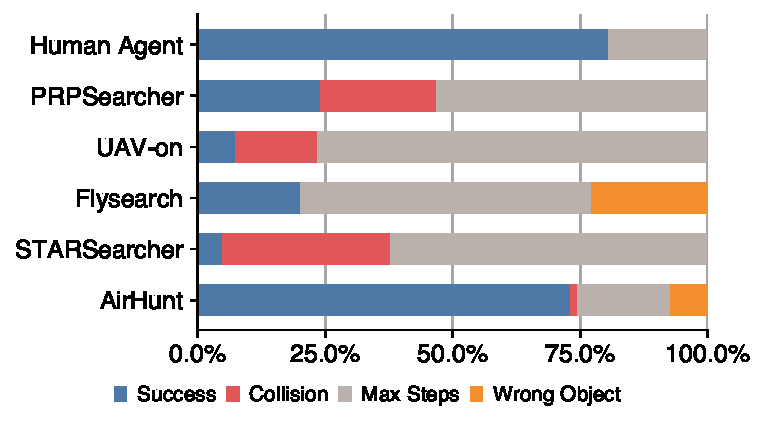
\includegraphics[width=0.98\linewidth]{figures/exp/error_breakdown-1.pdf}
    \caption{Failure Breakdown of \sysname and Baselines.}
    \label{fig:breakdown}
    \vspace{-15pt}
\end{figure}
\begin{figure}[t]
    \centering
    \setlength{\abovecaptionskip}{-8pt}  % 默认约为 10pt
    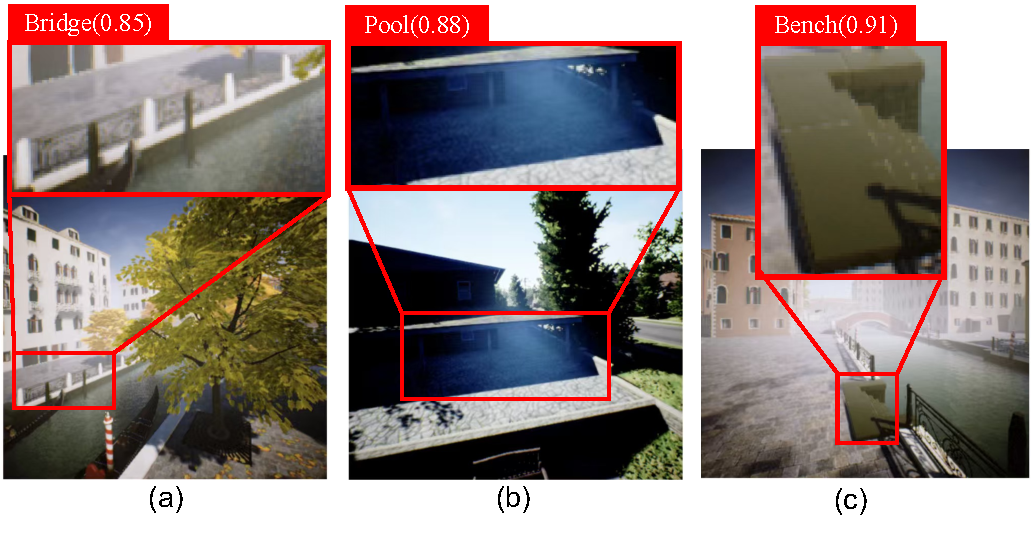
\includegraphics[width=0.98\linewidth]{figures/exp/wrongdetect.pdf}
    \caption{Examples of misclassification by object detectors. (a) A fence is misclassified as a bridge due to texture similarity. (b) A shadowed area is incorrectly detected as a pool. (c) A staircase is misidentified as a bench.}
    \label{fig:failedcase}
    \vspace{-8pt}
\end{figure}
\subsection{Failure Breakdown}
% flysearch有collision avoidance机制
We analyze and compare the failure reasons of all methods in the experiments, as illustrated in \fig\ref{fig:breakdown}. The categories include: \textit{Success}, indicating task completion; \textit{Collision}, referring to instances where the drone triggers a collision with an obstacle; \textit{Max Steps}, where the drone exceeds the maximum number of VLM queries without locating the target object; and \textit{Wrong Object}, where the drone stops in front of an incorrect object. As shown, the Human Agent achieves the best performance, closely followed by \sysname. Three key observations emerge from the analysis: 
(i) Baseline methods primarily fail due to exceeding the maximum steps. This is attributed to their over-reliance on VLM for decision-making, which often leads to inefficient exploration, as discussed in \S\ref{VI-B}; 
(ii) Most baselines exhibit considerable collision rates that would be unacceptable in real-world deployments where safety is critical. In particular, STARSearcher inspects every occupied surface at close distances, leading to frequent collisions with complex outdoor obstacles such as trees and thin lampposts. Other methods encounter collisions due to discrete motion primitives and inability to replan upon receiving new sensor observations. In contrast, \sysname substantially reduces collisions through elaborate planning, though it occasionally collides when exploring extremely narrow regions such as dense forests; 
(iii) Although our system is highly effective, it inherits certain limitations from object detector, Grounding-DINO~\cite{liu2024grounding}. As shown in \fig\ref{fig:failedcase}, the detector may hallucinate objects or misclassify background elements (e.g., shadows or fences) with high confidence due to texture ambiguity or lighting variations. This aligns with our real-world experiments, confirming that the primary bottleneck lies in the detector's sensitivity to visual noise.

\begin{figure*}[t]
    \centering
    \setlength{\abovecaptionskip}{-3pt}  % 默认约为 10pt
    
    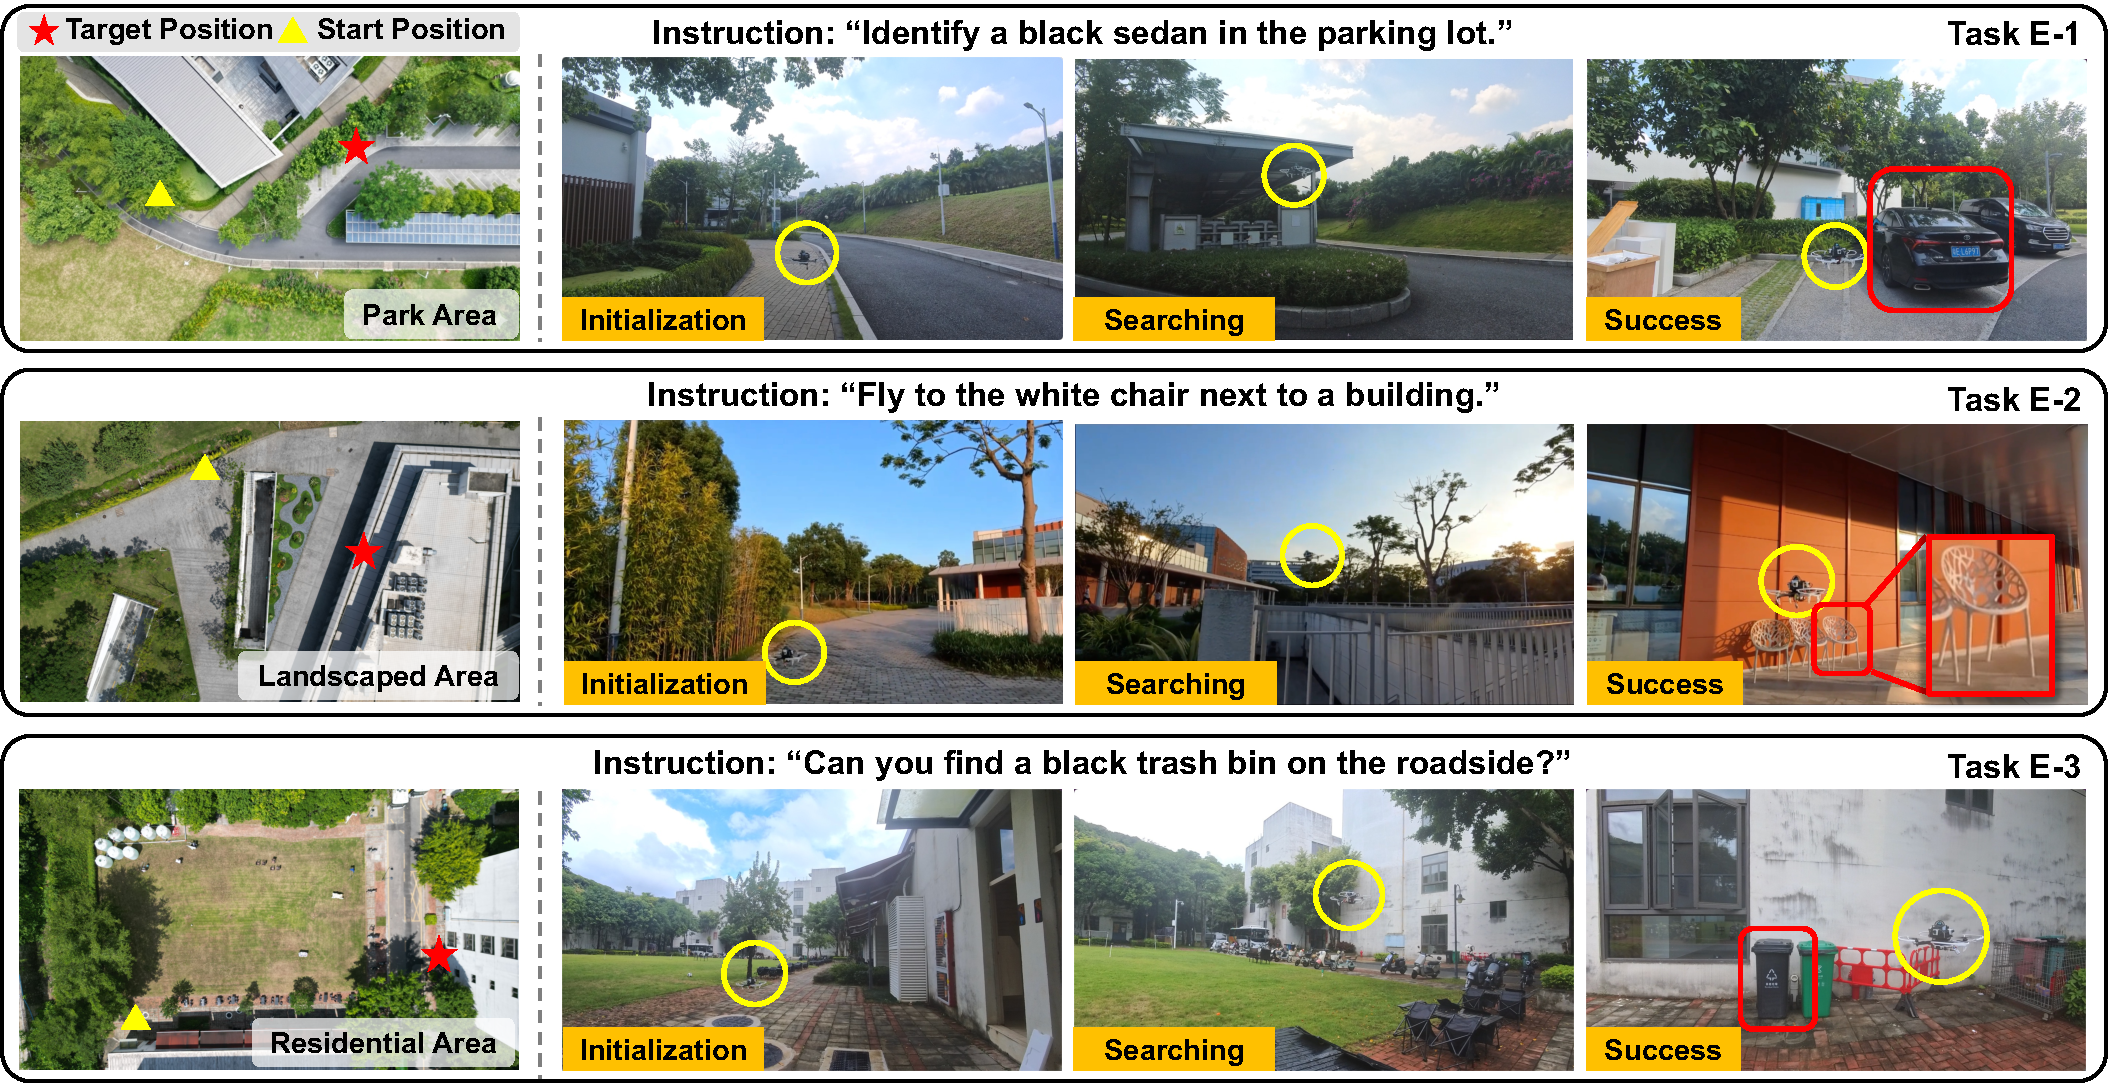
\includegraphics[width=0.98\linewidth]{figures/realdemo.pdf}
    \caption{Real-world experiments are conducted in three challenging environments, including a Park Area (E-1), a Landscaped Area (E-2), and a Residential Area (E-3). For each task, the first image illustrates a top-down view of the experimental scenario, and the others are snapshots of different drone states during task execution. The yellow circle marks the drone, and the red rectangles mark the target objects.}
    \label{fig:realworld}
    \vspace{-10pt}
\end{figure*}
\begin{figure}[t]
    \centering
    \begin{minipage}[t]{0.40\linewidth}
        \setlength{\abovecaptionskip}{-10pt}  % 默认约为 10pt

        \centering
        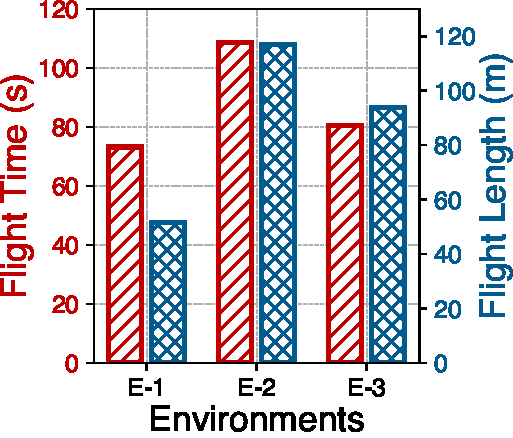
\includegraphics[width=0.98\linewidth]{figures/exp/results_rw.pdf}
        \caption{Total flight time and flight length in three real-world experimental tasks.}
        \label{fig:results_rw}
    \end{minipage}
    \hfill
    \begin{minipage}[t]{0.58\linewidth}
        \centering
        \setlength{\abovecaptionskip}{-10pt}  % 默认约为 10pt

        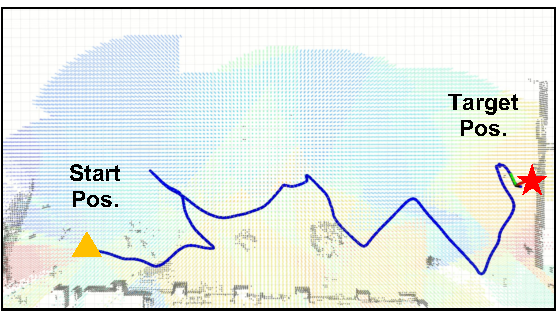
\includegraphics[width=0.98\linewidth]{figures/exp/traj.pdf}
        \caption{Example of drone's executed trajectory and value map in real-world experiments.}
        \label{fig:traj}
    \end{minipage}
    \vspace{-15pt}
\end{figure}
% \subsection{Real-world Experiments}
\section{Real-world Experiments}
% \noindent\textbf{Experimental Setup}
\subsubsection{Experimental Setup}
We conduct field experiments using a customized quadrotor platform equipped with an Intel NUC 11 Pro (8GB), a NxtPX4v2 autopilot, a Mid360 LiDAR, and three OAK-4P-New cameras with forward, left, and right orientations. The system operates under dynamics constraints of $v_{m}=1.0$m/s, $a_m=1.0$m/s$^2$, and $\omega=1.05$rad/s. We employ FAST-LIO~\cite{xu2021fast} for onboard localization and mapping. A ground station laptop communicates with the quadrotor and queries the online VLM via the 4G cellular network.


\begin{figure}[t]
    % \setlength{\abovecaptionskip}{-0.1cm} % height above Figure X caption
    % \setlength{\belowcaptionskip}{-0.4cm}
    \centering
    \setlength{\abovecaptionskip}{-5pt}  % 默认约为 10pt
    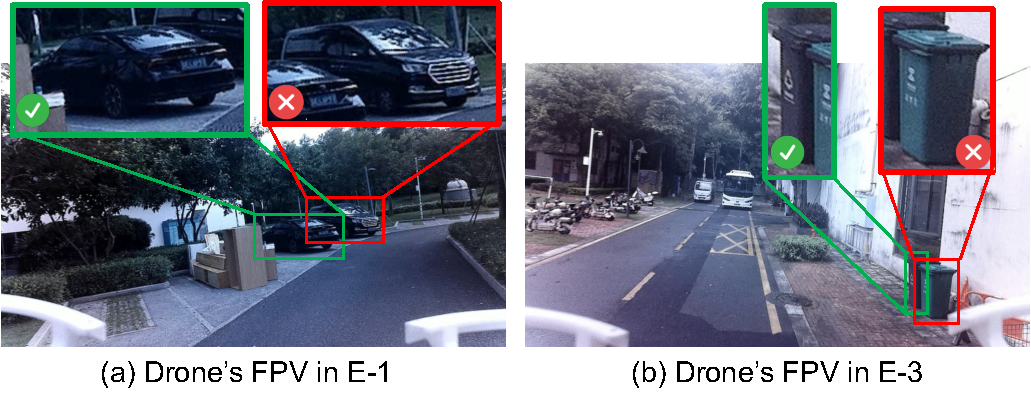
\includegraphics[width=0.98\linewidth]{figures/exp/droneFPV.pdf}
    \caption{Snapshots of the drone's FPV when detecting relevant objects in (a) E-1 and (b) E-3. (a) \sysname successfully identifies the target sedan (green box) and excludes the MPV car (red box), which is similar but incorrect. (b) \sysname correctly identifies the target black bin (green box) while excluding the green bin (red box).}
    \label{fig:fpv}
    \vspace{-10pt}
\end{figure}


We evaluate \sysname on three tasks in challenging outdoor environments with open-set instructions, as illustrated in Fig.\ref{fig:realworld}. These scenarios exhibit variations in environmental layout and navigational context, with distinct spatial characteristics including obstacle density, open space ratio, and terrain elevation. Specifically,
\textbf{Task E-1} is conducted in a park area with residential buildings, tree-lined curved streets, and parking spaces. The drone navigates from a complex intersection to locate a black sedan.
\textbf{Task E-2} is performed in a landscaped area with obstacles including walls and barriers. The drone starts from a position adjacent to a barrier to locate a white chair.
\textbf{Task E-3} takes place in a residential zone with a spacious grassy field surrounded by roads. The drone starts from a corner of the grassland to locate a black trash bin.

\subsubsection{Quantitative Results}
\fig\ref{fig:results_rw} summarizes the quantitative performance of \sysname across all experimental scenarios. The system successfully completes navigation tasks in tasks E-1, E-2, and E-3 with flight times of 73.2s, 108.5s, and 80.5s, respectively. The example trajectory illustrated in \fig\ref{fig:traj} demonstrates continuous execution with minimal detours and limited revisits to previously explored regions, resulting in efficient navigation with short flight durations and distances. This efficiency can be attributed to our SGCP module, which fuses geometric information and semantic cues to generate consistent trajectories.

\subsubsection{Qualitative Results}
We present the experimental scenes and the navigation process from initialization through searching to task completion, demonstrating successful target localization in all scenarios based on given instructions (\fig\ref{fig:realworld}). \fig\ref{fig:fpv} further illustrates snapshots of the drone's first-person view when detecting objects relevant to the given instructions. \sysname's ADTR module incorporates a robust object verification mechanism that successfully excludes visually similar but semantically incorrect objects and identifies the correct target that matches the semantic context in the instructions. This verification capability contributes to increased navigation success rate in complex real-world environments. In summary, these results validate \sysname's superior object navigation capabilities in large-scale outdoor environments. Detailed experimental results and additional visualizations are provided in the Supplementary Material.








